This section describes the User interface of the BBP system, offering a glimpse into the
various pages that constitute the application The design mockups presented here prioritize
the interaction dynamics rather than the final aesthetic design, recognizing that visual
elements may get adjustments during the testing phase, as outlined in the RASD.

\section{Overview}

\begin{figure}[htbp]
	\centering
	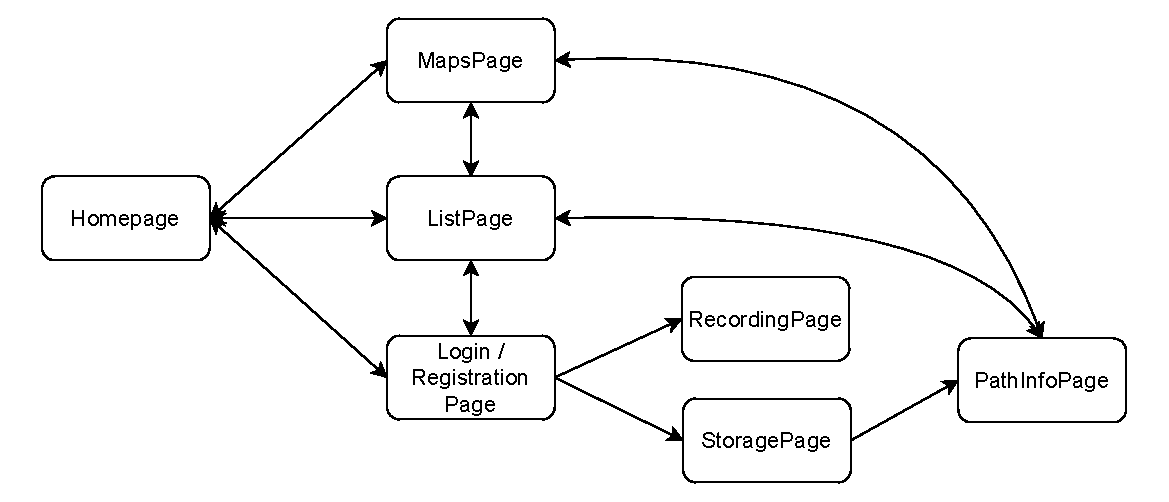
\includegraphics[width=\textwidth]{Images/UIOverview.drawio.pdf}
	\caption{User Interface Overview}
\end{figure}

The figure serves as a high-level representation of the user interface navigation flow within the Best Bike Paths (BBP) application. 
It illustrates the logical interconnections between the primary screens, positioning the Homepage as the central hub for user interaction. 
The diagram delineates the pathways to general discovery features, such as the MapsPage and ListPage, while identifying the Login/Registration Page 
as the critical gateway for accessing authenticated functionalities, specifically the RecordingPage and StoragePage. The PathInfoPage is a convergent
destination accessible from multiple views, ensuring users can retrieve detailed route information regardless of their entry point. 
A more granular analysis of these specific pages and their respective functional components will be provided in the subsequent paragraphs.

\newpage
\subsection{Dock}

\begin{figure}[htbp]
	\centering
	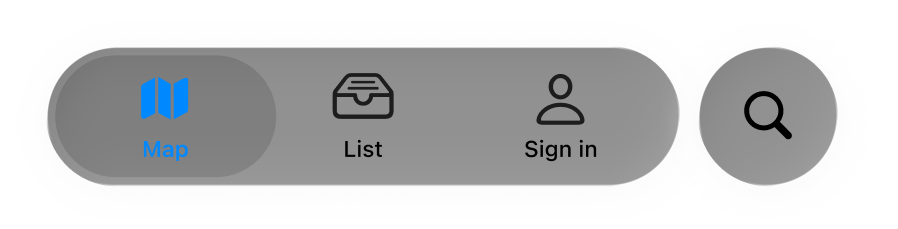
\includegraphics[width=\textwidth]{Images/Dock.png}
	\caption{Dock}
\end{figure}

The user interface features a persistent navigation dock located at the bottom of the screen, ensuring consistent and rapid access to the application's 
primary sections regardless of the currently active view. This central component is structured to house shortcuts to core functionalities: the geospatial 
visualization (Map), the textual list of available paths (List), and the authentication or profile management area (Sign in / Account). Adjacent to the main 
navigation module, a dedicated circular button allows for the immediate activation of the global search function (Search), thereby optimizing the user experience 
for the quick retrieval of specific routes.

\newpage
\subsection{User Interface}

\subsubsection*{MapsPage}
\begin{figure}[H]
    \centering
    \includegraphics[page=1, width=0.28\textwidth]{mockup.pdf}
    \caption{Home screen with map view showing available bike paths}
\end{figure}

The figure above illustrates the application's Home screen, which serves as the primary entry point for the Best Bike Paths (BBP) system. Upon launching, 
the interface immediately renders an interactive map centered on the user's current geolocation, visualizing the surrounding network of bike paths. 
These routes are dynamically filtered and prioritized based on their proximity to the user and their aggregate quality rating, ensuring that the most relevant and "optimal" paths 
are highlighted effectively.

From a user experience perspective, a key architectural decision was to maintain interface uniformity; this screen is functionally identical for both Guest Mode and Authenticated User Mode, 
the only difference is the presence of the recording button in the top right corner. This design choice ensures that the core value proposition of the system, the discovery of safe bike paths—is 
immediately accessible to all users without requiring a login barrier.

Graphically, the interface prioritizes a "map-first" design to maximize spatial awareness. This approach prevents visual clutter, ensuring that the navigational map remains the 
focal point while the bottom navigation bar provides distinct access to the Map, List view, and Account settings.

\newpage
\subsubsection*{ListPage}
\begin{figure}[H]
    \centering
    \includegraphics[page=3, width=0.28\textwidth]{mockup.pdf}
    \caption{List view of available bike paths filtered by proximity or rating}
\end{figure}

The figure illustrates the "List of Paths" interface, which serves as a structured, data-centric alternative to the map visualization for browsing available cycling routes. Consistent with the 
application's unified design philosophy, this view allows both Guest and Authenticated users to access the same repository of community-generated paths, ensuring the public utility of the system is 
maintained across all access levels.

From a design perspective, the interface adopts a clean, vertical list layout intended to facilitate rapid scanning and comparison of multiple routes. Each entry is hierarchically organized to 
prioritize the route's topology (Origin and Destination), followed immediately by quantitative metrics such as estimated duration and total distance.

\newpage
\subsubsection*{AuthenticationPage}
\begin{figure}[H]
    \centering
    \includegraphics[page=4, width=0.28\textwidth]{mockup.pdf}
    \caption{Authentication screen: Login and Sign-up forms}
\end{figure}

The figure depicts the Authentication Interface, which acts as the gateway for users to transition from the limited Guest Mode to a fully privileged Registered User session. Visually, the interface 
maintains contextual continuity by utilizing a blurred version of the main map view as the background. This design choice subtly reinforces the application's geospatial focus while ensuring that the 
foreground elements—specifically the "BBP" branding and the credential input fields, whichs remain the primary visual focus to minimize user distraction.

Functionally, the screen is designed to streamline the entry process for both returning and new users. It features standard input fields for email and password, followed by a distinct visual 
hierarchy for action buttons: the "Sign In" command is emphasized in the system's primary blue color to encourage the most common action, while the "Sign Up" option is presented neutrally. 
Notably, the persistence of the bottom navigation bar demonstrates a non-blocking architectural approach; the authentication state is accessible via the "Sign in" tab, allowing users to freely navigate 
back to the "Map" or "List" views without being locked into a login loop, thereby preserving the application's "Guest First" accessibility philosophy.

\newpage
\subsubsection*{ProfilePage}
\begin{figure}[H]
    \centering
    \includegraphics[page=6, width=0.28\textwidth]{mockup.pdf}
    \caption{Profile Screen: User account details and history of recorded trips}
\end{figure}

The figure depicts the User Profile Interface, which serves as the central dashboard for authenticated users to manage their personal data and review their activity log. Upon successful login, 
the system presents this personalized view, prominently displaying the user's identity and aggregate performance metrics, such as the total cumulative distance cycled. Crucially, this interface functions 
as the primary entry point for the Personal Trip Storage, acting as a digital repository for the user's historical route data. The "Your last 3 trip" section offers a chronological summary of recently completed rides, 
providing key details for each entry: origin, destination, duration, and specific path conditions. This design ensures that users can easily retrieve and analyze their past cycling performance while maintaining quick 
access to the rest of the application via the navigation bar.

\newpage
\subsubsection*{ManualInputPage}
\begin{figure}[H]
    \centering
    \includegraphics[page=7, width=0.28\textwidth]{mockup.pdf}
    \caption{Manual Input: Interface for manually adding a new bike path or segment}
\end{figure}

The figure illustrates the Manual Path Registration Interface, designed to support the "offline reporting" workflow where users reconstruct a route after completing a ride. This screen is essential for data collection 
when real-time tracking is not utilized, allowing registered users to manually input trip details. The interface is structured to first capture high-level metadata, requiring the user to specify the "From" and "To" points, 
along with the precise start and end times to establish the temporal context of the trip. Below this, the "Streets of the path" section allows for a granular reconstruction of the route topology; users can sequentially add 
the specific street segments traversed. A key feature of this view is the ability to annotate individual segments with condition reports—such as the presence of "Potholes". The user can then confirm the entry via the "Confirm" button.

\newpage
\subsubsection*{PathDetailsPage}
\begin{figure}[H]
    \centering
    \includegraphics[page=11, width=0.28\textwidth]{mockup.pdf}
    \caption{Path Details: Comprehensive data and statistics for a specific bike route}
\end{figure}

The figure illustrates the Path Details Interface. Visually, the screen is anchored by a top-level map widget that isolates the selected path geometry, offering immediate spatial context regarding the route's trajectory. 
Below this, the layout prioritizes critical quantitative data, specifically the origin, destination, total distance, and estimated duration, presented in a clean, high-legibility typography. 
A central component of this view is the display of the proprietary Path Score, which aggregates road surface quality and user feedback into a single metric. This is paired with a prominent safety alert mechanism that explicitly 
highlights specific hazards, such as reported potholes, using cautionary color coding (orange) to ensure user awareness of potential risks. Finally, the interface provides a textual breakdown of the route topology by listing the 
specific sequence of streets comprising the path, enabling users to cross-reference the digital route with their local knowledge.

